% !TEX program = lualatex
\documentclass[aspectratio=43,professionalfonts,handout]{beamer}
\usepackage{beamer_template}

\newcommand{\LectureNum}{14}
\newcommand{\LectureTitle}{問題演習}
\newcommand{\TextPages}{p.\,98-100（練習問題2-A, 2-B）}
\newcommand{\NextTopic}{前期復習}
\newcommand{\NextPages}{p.\,72-100}
\newcommand{\CourseName}{基礎数学B}
\renewcommand{\TermName}{前期}

\begin{document}

% -----------------------------------------------
% スライド1: 表紙＋目標＋用語・定義
% -----------------------------------------------
\begin{frame}{\CourseName\quad 第\LectureNum 回「\LectureTitle 」}
  {\small \TermName\quad \TeacherName\quad ／\quad 教科書 \TextPages\quad
  \textbf{目標}：べき関数・分数関数・無理関数・逆関数を総合的に理解する}

\end{frame}

% -----------------------------------------------
% スライド2: 公式・性質
% -----------------------------------------------
\begin{frame}{公式・性質}
  \begin{block}{}
  \begin{itemize}
    \item % TODO: 内容を追加
  \end{itemize}
  \end{block}
\end{frame}

% -----------------------------------------------
% スライド3: 図・グラフ（TikZコードを手動追加）
% -----------------------------------------------
\begin{frame}{図・グラフ}
  \centering
  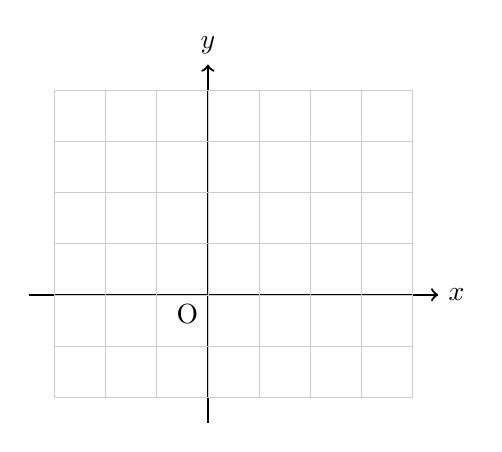
\begin{tikzpicture}[scale=0.65]
    \draw[->,thick] (-3.5,0) -- (4.5,0) node[right]{$x$};
    \draw[->,thick] (0,-2.5) -- (0,4.5) node[above]{$y$};
    \node[below left] at (0,0) {O};
    \draw[gray!40, very thin] (-3,-2) grid (4,4);
    % ここにグラフを描画
  \end{tikzpicture}
\end{frame}

% -----------------------------------------------
% まとめ
% -----------------------------------------------
\begin{frame}{まとめ}
  \begin{itemize}
    \item べき・分数・無理関数はすべて「グラフの形」と「定義域・値域」がセット
    \item 逆関数は定義域の確認を忘れずに
    \item 練習問題で各関数の特徴を整理する
  \end{itemize}
\end{frame}

\end{document}
